\documentclass[
	letterpaper, % Paper size, specify a4paper (A4) or letterpaper (US letter)
	10pt, % Default font size, specify 10pt, 11pt or 12pt
]{CSUniSchoolLabReport}

%----------------------------------------------------------------------------------------
%	REPORT INFORMATION
%----------------------------------------------------------------------------------------

\title{Lab Four\\ Power Systems Analysis \\ EECE5682} % Report title

\author{Michael \textsc{Brodskiy}\\ \small \href{mailto:Brodskiy.M@Northeastern.edu}{Brodskiy.M@Northeastern.edu}}

\date{October 24, 2024} % Date of the report

%----------------------------------------------------------------------------------------


\begin{document}

\maketitle % Insert the title, author and date using the information specified above

\begin{center}
	\begin{tabular}{l r}
		Date Performed: & \today \\ % Date the experiment was performed
		Instructor: & Professor \textsc{Abur} \\ % Instructor/supervisor
	\end{tabular}
\end{center}

\newpage

\begin{abstract}

  This laboratory experiment explores three phase transformers in both voltage magnitude shifting and phase shifting applications. The simulated three phase circuits were balanced, and contained regulating transformers used to modify real and reactive power flow, as well as voltages.

\end{abstract}

\begin{flushleft}

  \textsc{Keywords:} \underline{three phase transformer}, \underline{magnitude shifting}, \underline{phase shifting}, \underline{regulating}, \underline{power flow}

\end{flushleft}

\newpage

\section{Introduction \& Objectives}

We begin by constructing a three-phase phase shifter as follows:

\begin{figure}[H]
  \centering
  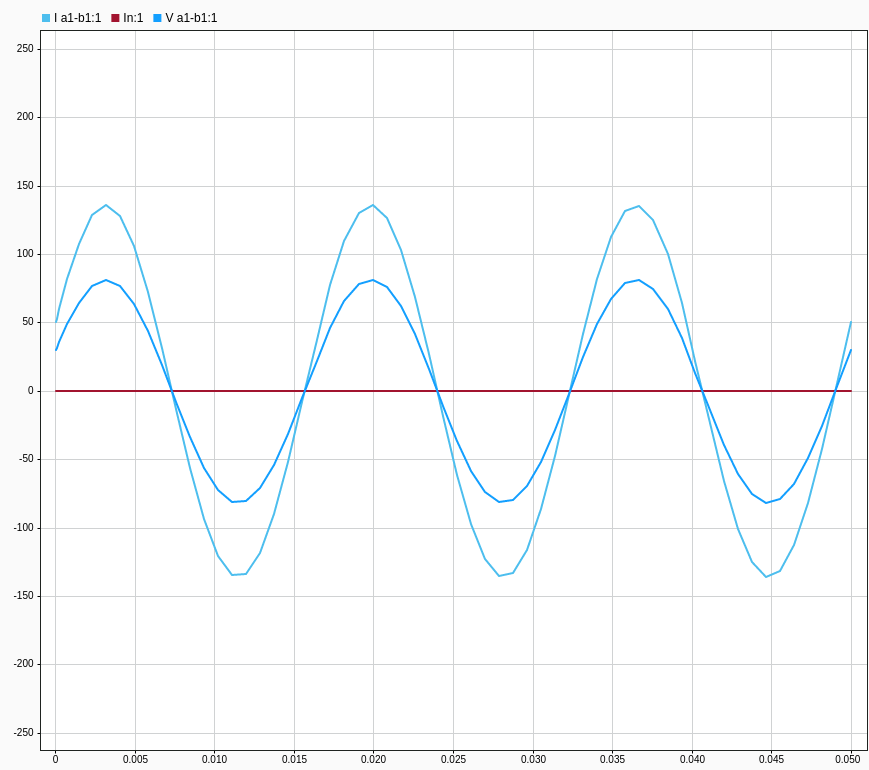
\includegraphics[width=.9\textwidth]{Figures/Lab\ Four/Parta}
  \caption{Initial Circuit Construction (Part A)}
  \label{fig:1}
\end{figure}

This circuit was then used to simulate the conditions indicated below.

\section{Results \& Analysis} 

\subsection{Part B: Simulating with Ratio $V^n:\Delta V^n\to 100:.01$}

In the initial case, $V^n:\Delta V^n$ was simulated as $100:.01$. This produced the following output:

\begin{figure}[H]
  \centering
  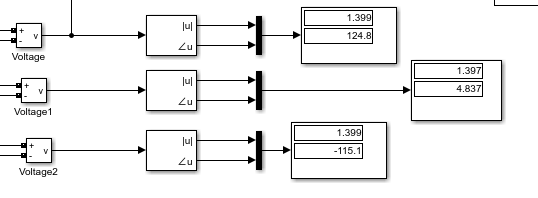
\includegraphics[width=.75\textwidth]{Figures/Lab\ Four/Partb1}
  \caption{Secondary Line Voltage Magnitude and Phase Angle}
  \label{fig:2}
\end{figure}

\begin{figure}[H]
  \centering
  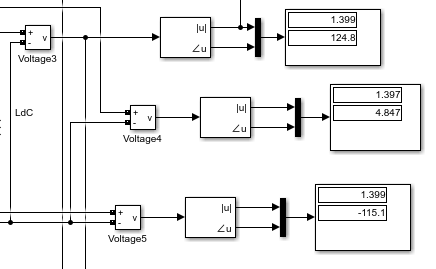
\includegraphics[width=.75\textwidth]{Figures/Lab\ Four/Partb2}
  \caption{Primary Line Voltage Magnitude and Phase Angle}
  \label{fig:3}
\end{figure}

We may observe that the phases are near-identical. Measuring the real and reactive power flows through each line, we may find:

\begin{figure}[H]
  \centering
  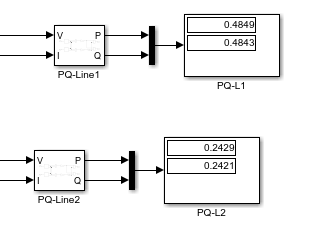
\includegraphics[width=.5\textwidth]{Figures/Lab\ Four/Partb3}
  \caption{Real/Reactive Power Flows (Primary Line Top, Secondary Line Bottom)}
  \label{fig:4}
\end{figure}

We may, however, observe that the real and reactive power flows through the primary line are near double those of the secondary line, in per-unit.

\subsection{Part C: Simulating with Ratio $V^n:\Delta V^n\to 100:3$}

For the second case, $V^n:\Delta V^n$ was simulated as $100:3$. This produced the following output:

\begin{figure}[H]
  \centering
  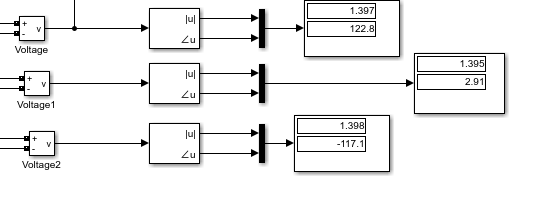
\includegraphics[width=.75\textwidth]{Figures/Lab\ Four/Partc1}
  \caption{Secondary Line Voltage Magnitude and Phase Angle (100:3)}
  \label{fig:5}
\end{figure}

\begin{figure}[H]
  \centering
  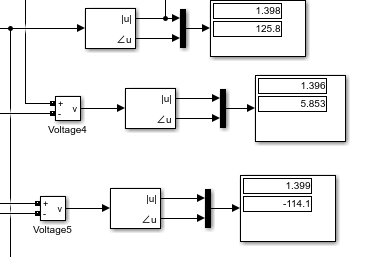
\includegraphics[width=.75\textwidth]{Figures/Lab\ Four/Partc2}
  \caption{Primary Line Voltage Magnitude and Phase Angle (100:3)}
  \label{fig:6}
\end{figure}

We may observe that the phases now shift much more than in the initial case, with each phase in the secondary line lagging the phases in the first by about $3^{\circ}$. Measuring the real and reactive power flows through each line, we may find:

\begin{figure}[H]
  \centering
  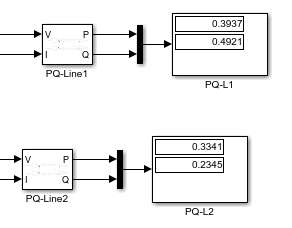
\includegraphics[width=.5\textwidth]{Figures/Lab\ Four/Partc3}
  \caption{Real/Reactive Power Flows (Primary Line Top, Secondary Line Bottom, Voltage Ratio 100:3)}
  \label{fig:7}
\end{figure}

From the initial case, we may observe that the real power flows are much closer, while the ratio of reactive power flow between the primary and secondary line is even greater than two.

\section{Conclusion}

\begin{enumerate}

  \item For the phase regulating transformers, we may see that, in the initial case, the line voltage magnitudes and phases were near identical; however, the power flows in the primary line were double those of the second line. On the other hand, in the second case (100:3), the magnitudes were the same, but the phases differed by nearly $3^{\circ}$ (the secondary line lagged). For the power, we see that the initial case had double the real and reactive power flow on the primary line as the secondary, while the ratio for the real power decreased, while it increased for the reactive for the second case. As such, since the ratio decreased by a lot, \underline{we may conclude that the real power is greatly affected by changes} \underline{in the phase}. We may conclude that this is because, for real power flow, the conductances and susceptances (which are multiplied by trigonometric functions of the angle), are summed, while they are subtracted for reactive power flow. Increasing the angle thus increases the value of the $\sin$ and decreases the $\cos$, which leads to this result.

\end{enumerate}

\end{document}
